\section{Data: Reddit as a community}

We start with a brief overview of both Reddit and the dataset that we use in this paper, focusing on aspects that directly impact our analyses\footnote{There is much more to say about both Reddit itself (see \url{https://www.reddit.com/about/}) and the dataset (see 
\url{https://news.ycombinator.com/item?id=9869871}.

\subsection{What is Reddit, briefly}

%% DC 10: Will want a couple of legible screenshots here to help illustrate.
Reddit is one of the largest sharing and discussion communities on the Web.  According to Alexa, as of late 2015 Reddit is in the top 15 sites in the U.S. and the top 35 in the world in terms of monthly unique visitors.  It consists of a large number of subreddits (X as of DATE), each of which focuses on a particular purpose.  Many subreddits are primarily about sharing web content from other sites: in ``Pics'', ``News'', ``Funny'', ``Gaming', and many other communities, users (``Redditors'') make ``submissions'' of links posted at other sites that they think are interesting.  In other subreddits, Redditors primarily write text-based ``self-posts'': ``AskReddit'', ``IamA'', ``ShowerThoughts'' are places where people can ask questions and share stories of their own lives.  Generically, we will refer to submissions and text posts as ``submissions''.  

%% DC 10: Sam should choose a precise terminology here and use it throughout, and be clear on every single analysis exactly what is being counted.  We don't want someone being confused, trying to replicate the data, and finding something different because they don't understand what the analysis is.  (We will also want to be super-clear below when we introduce the dataset to talk about any filtering we did, so that people can exactly replicate what we did.)

%% DC 10: Further, this terminology should agree with Reddit's, so that people who are familiar with the community aren't confused. 

Each post can be imagined as the root of a threaded comment tree; in addition to posting, Redditors can make comments, and vote on both posts and comments.  Votes are used both to sort comments within a post and posts within a subreddit, and also form the basis of ``karma'', a reputation system that essentially tracks how often people upvote a given Redditor's comments and submitted links.  Redditors can also create and volunteer to moderate subreddits.

We choose Reddit as our target community for a number of reasons.  It has existed since 2007, meaning that there has been ample time for the community to evolve and for differences in user cohorts to appear.  Second, being composed of a number of diverse subreddits allows us to explore questions of how communities diverge over time.  Third, Reddit data are publicly available through an API.

\subsection{The dataset}

Redditor Stuck_In_The_Matrix used the API to compile a more-or-less complete dataset of posts and comments since the inception of Reddit on XXXX.  This dataset is publicly available via...

%% DC 10: Sam, you gotta fill this out; I don't know the story.

%Amit 9: How was the data made available? Good to explain a little about the source.

We focus on submissions and comments in the dataset because they have timestamps and can be tied to specific users and subreddits, allowing us to perform our time-based analyses.   In some analyses, we look only at comments; in some, we combine comments and submissions, calling them ``posts''.  We would also like to have looked at voting behavior as a measure of user activity\footnote{Which would also give us more insight than usual into lurkers' behavior; we'll return to this in the discussion.}, but individual votes with timestamps and voting user are not available through the API, only the aggregate number of votes that posts receive.
%% DC 10: Adding a note that we know we're ignoring lurkers, both because it's actually important to note that and to avoid being crushed by reviewers who care about lurking.
%%


\subsection{Our processing}

XXXX How did we process the dataset, both technically (using the existing BigQuery access, making our own tables), and in terms of filtering?

%% DC 10: Can we also please get rid of 2007 in all the figures?  It appears that 
\subsection{An overview of the dataset}

%% DC 10: Aga
Figures~\ref{fig:cumulative_users_subreddits}~and~\ref{fig:active_users_subreddits} show an overview of Reddit's growth over time.  

Figure~\ref{fig:cumulative_users_subreddits} shows the cumulative number of user accounts and subreddits created over time as of the last day of every month, along with the ratio between them.  After an initial extremely rapid expansion from 2008--2009, both the number of users and subreddits have grwen exponentially.  As of the end of 2014, about 16.2 million distinct users have made at least one comment and 327,000 subreddits received at least one comment since Reddit's inception.
%% DC 10: Assuming because you say comment you really mean "comments".  That's fine (though I wonder if it would make more sense in the overview for both this and for active to combine both posts and comments as "activity")

%% DC 10: Unless the ratio has useful analysis to be done, we should get rid of it as noise.

%% DC 10: I tike that the figure axes are much more legible.  But, things still to fix: Axes should be meaningful labels: "Average posts per user". "Total Created".  "Total Active Per Month".  Figures should have legend items in the same vertical order as data series, and the series should also probably be drawn not just with colors but with different patterns, to faciliate their reading in black and white.  Charts with a single data series probably don't need a legend (which should just be embedded in the caption).  This should get fixed throughout once we've decided exactly which figures to keep.
\begin{figure}[!tb]
\centering
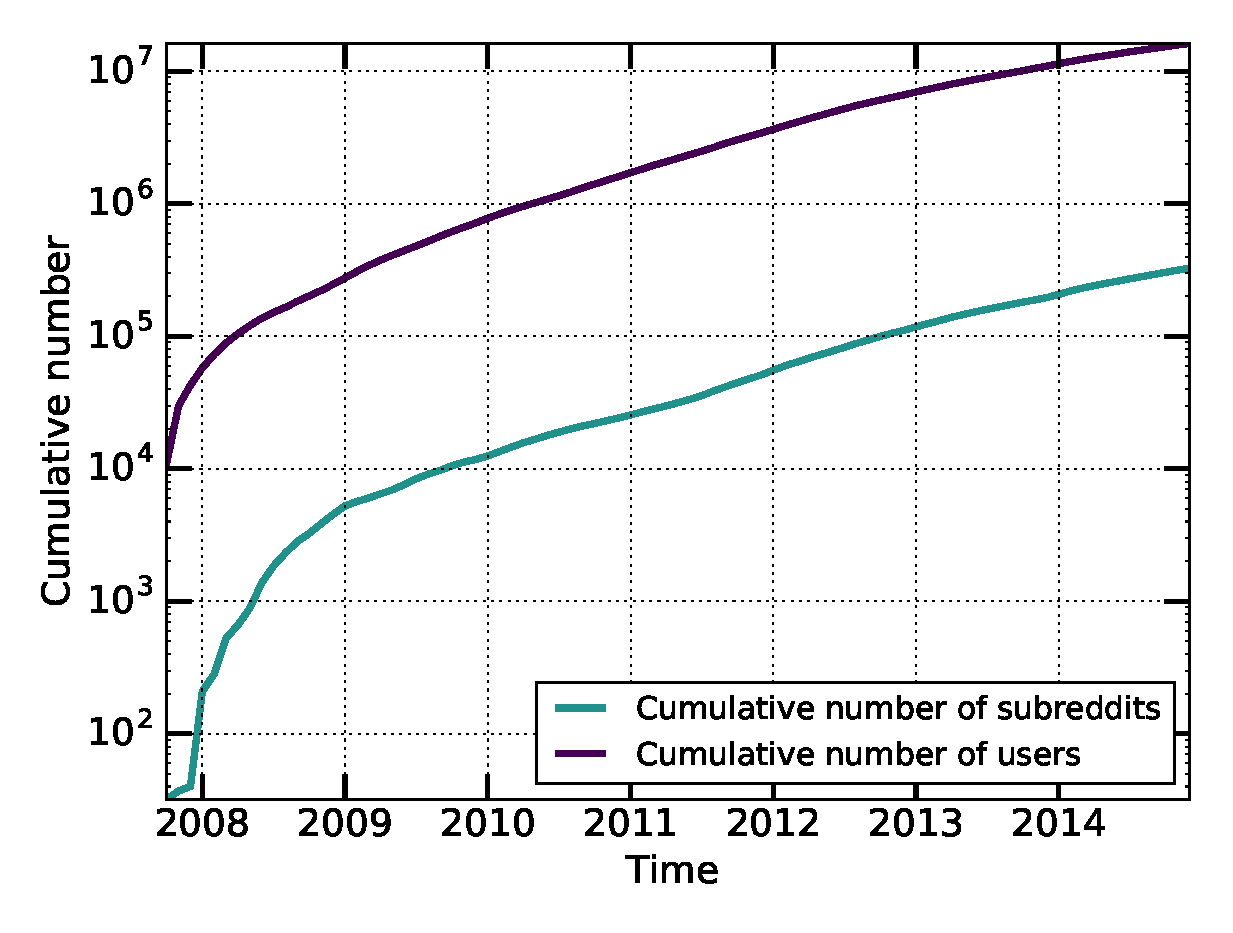
\includegraphics[scale=0.4]{./images/cumulative_users_subreddits.eps}
\caption{Caption}
\label{fig:cumulative_users_subreddits}
\end{figure}

%% DC 10: Since there can be redditors that only submit and don't comment, if this is really comments then it understates activity -- so I am now even more convinced that this should be combined submissions and comments.
%% Sam 10: The active subreddits and user accounts are all based on the joint submission and comment behavior.
However, as with many other online sites, most users \cite{} and communities \cite{butler/kraut paper} do not stay active.  Figure~\ref{fig:active_users_subreddits} shows the monthly number of user accounts and subreddits that received at least on comment.  In December 2014, about 470,000 thousand users made comments and about 11,400 subreddits received comments; both are an order of magnitude less than the cumulative number of users or subreddits.  

\begin{figure}[!tb]
\centering
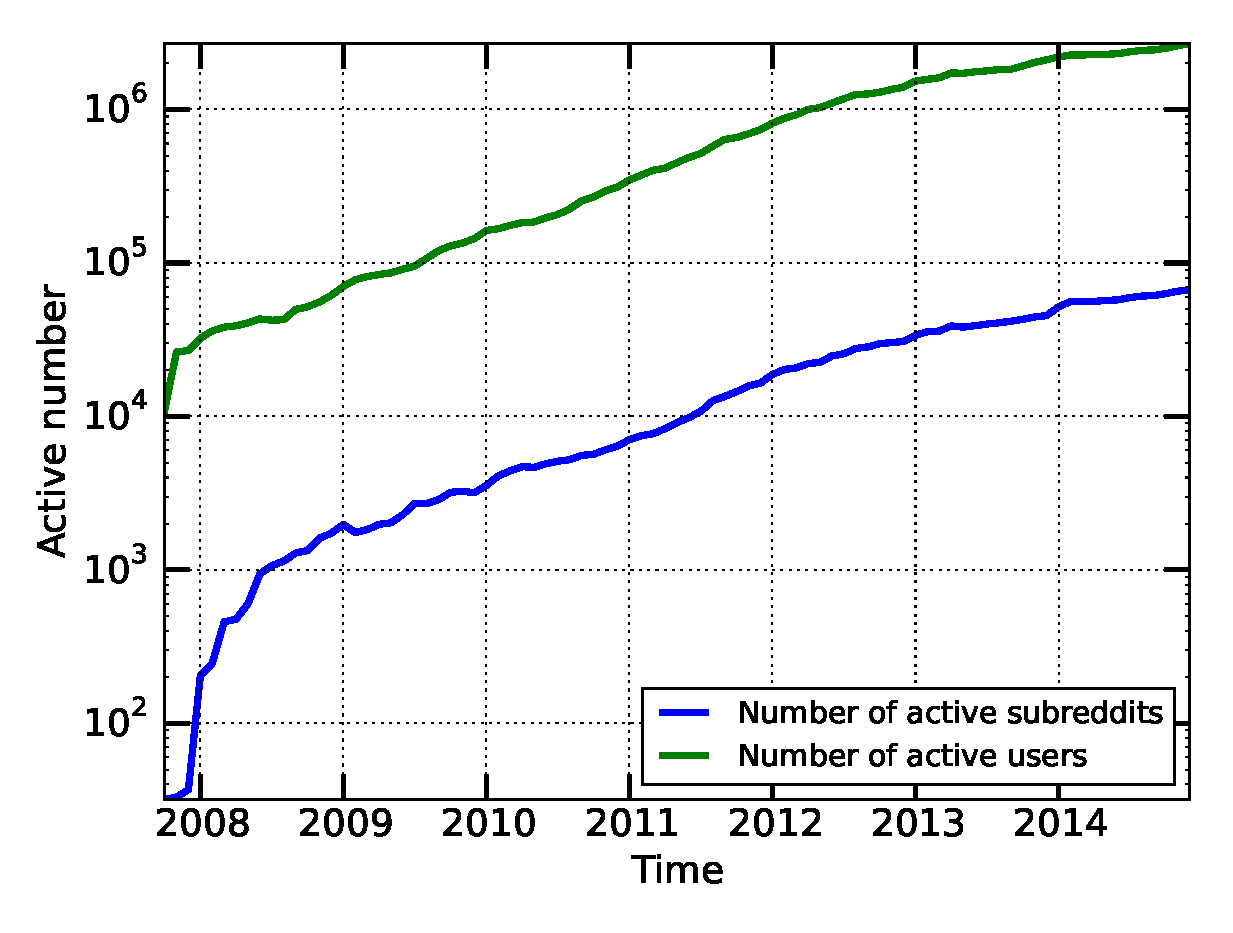
\includegraphics[scale=0.4]{./images/active_users_subreddits.eps}
\caption{Caption}
\label{fig:active_users_subreddits}
\end{figure}


The fact that such a significant amount of users stopped using the platform raises questions such as why users give up on their accounts, when they do so and which users are more likely to stay active. 

\subsection{Identifying cohorts}
%% DC 10: Trying to decide whether this works better here or at the beginning of a cohorty section -- there is some subtlety that I think Sam wants to work through when introducing the first problem.
%% Amit 9: Added this subsection here. Having the cohorts defined as the part of the overview will help, as we talk about them throughout the paper. Some of the cohort stuff from next section can come here. 
